% !TEX root = tracking.tex
\section{General Framework \label{sec:framework}}
Given a dynamical system, we propose a hierarchical framework for combining Hamilton-Jacobi safety analysis with planning methods in a modular way.

Given: Target, mechanism for sensing obstacles

Goal: reach target without colliding with obstacles

Offline: compute bubble and error-feedback controller (tracker)

Online: At every time iteration,
\begin{enumerate}
  \item Sense and update obstacles (can also be done every N iterations)
  \item Augment obstacles according to bubble
  \item Plan path or trajectory using planner, assuming currently sensed and augmented obstacles
  \item Robustly track trajectory using tracker
\end{enumerate}


\textbf{Maybe put next paragraph in the introduction}

There are many fast planners that could potentially do planning in real-time; however, these typically cannot account for disturbances in a provably safe way. In addition, complex system models with nonlinear dynamics complicate planning algorithms (non-convex for MPC, more difficult for RRT). On the other hand, HJ reachability is able to handle disturbances, and is agnostic to system dynamics. In addition, provably guarantees can be provided. However, HJ reachability and in general formal verification methods can be very expensive to compute.

Refer to figure: planning level and safety level. 

In the safety level, we start with the error dynamics, and we compute two things: bubble which is fed into planner to plan with extra margin, and error-feedback controller for real-time control. These two can be computed offline independent of the planned path.

In the planning level, any planning method such as MPC, RRT, etc. (cite some things) can be used. The planning level does not need to take into account disturbances, and can use simple system dynamics or even no dynamics at all. In fact we will be using a simple RRT planner which simply provides paths, in the form of a sequence of line segments, which are not dynamically feasible. 

\begin{figure}
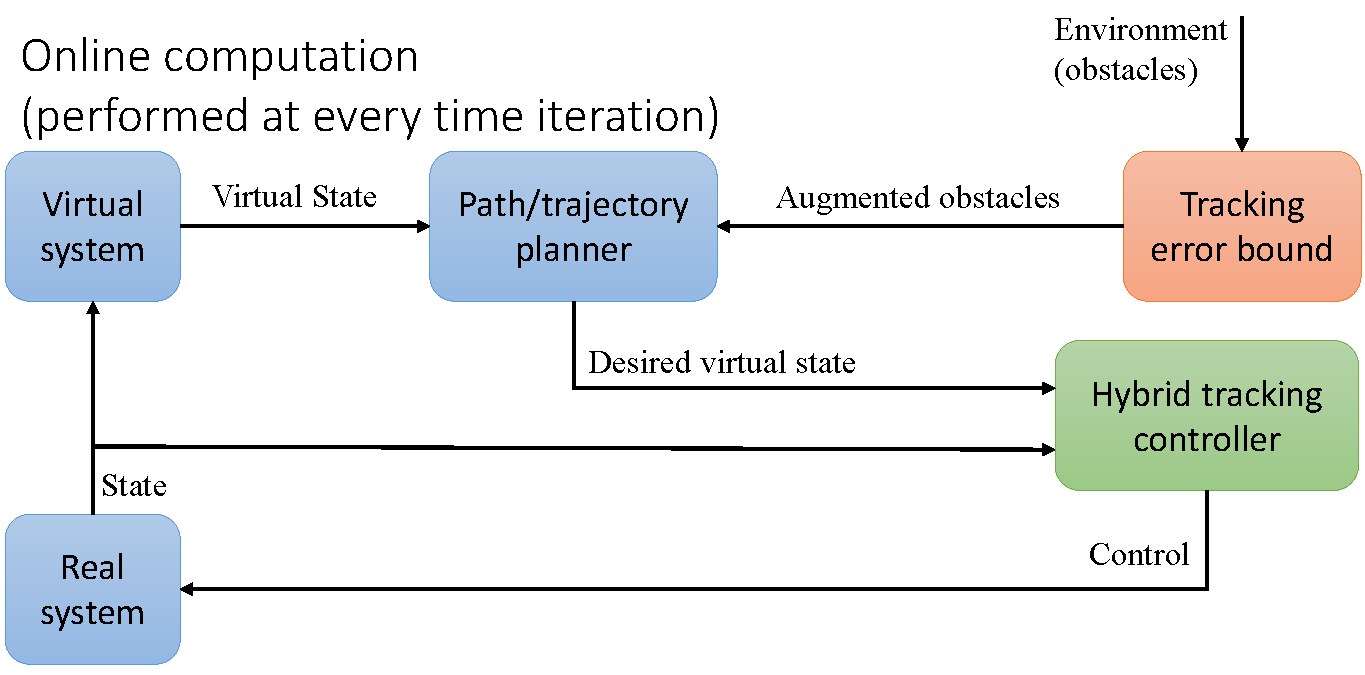
\includegraphics[width=\columnwidth]{fig/framework_online}
\caption{Online framework}
\label{fig:fw_online}
\end{figure}

\begin{figure}
  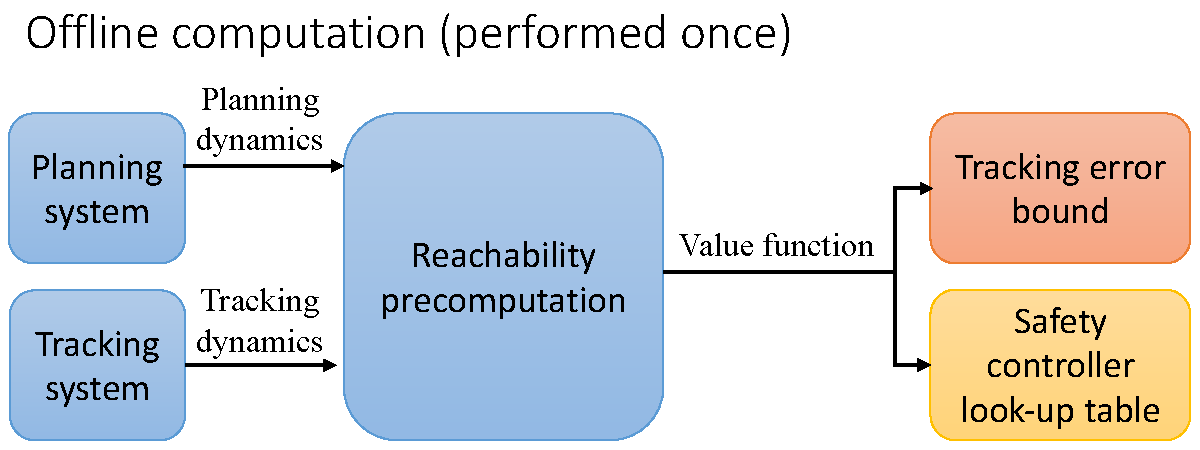
\includegraphics[width=\columnwidth]{fig/framework_offline}
  \caption{Offline framework}
  \label{fig:fw_offline}
\end{figure}

\begin{figure}
  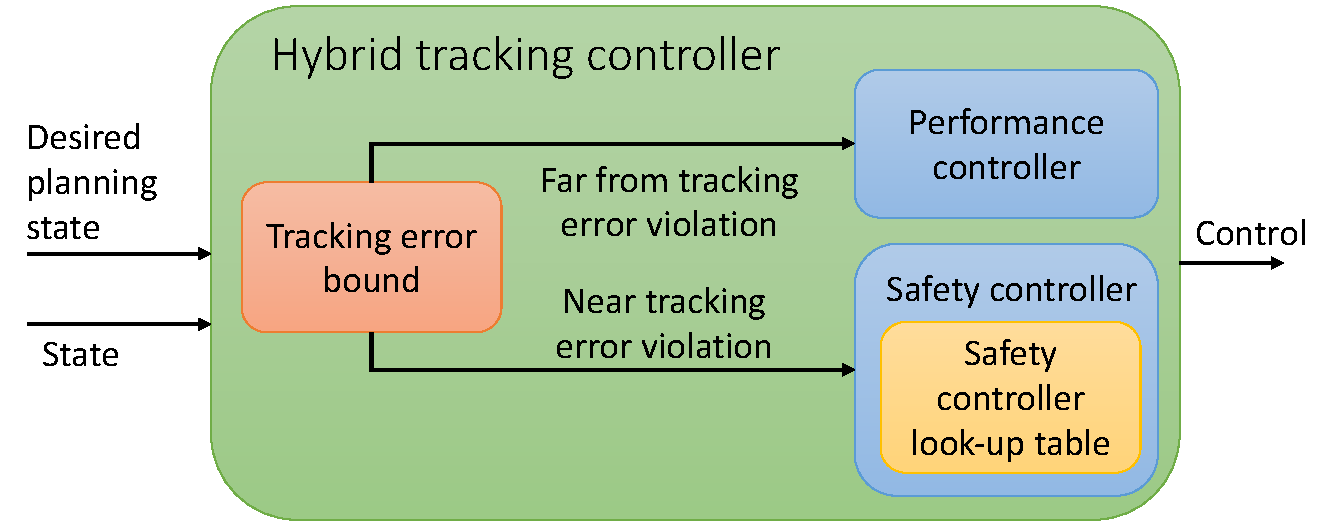
\includegraphics[width=\columnwidth]{fig/hybrid_controller}
  \caption{Hybrid controller}
  \label{fig:hybrid_ctrl}
\end{figure}